\documentclass[%
12pt,                % Schriftgröße
paper=a4,            % Papiergröße
captions=tableabove, % Beschriftungen für Tabellen oberhalb
]{scrartcl}

% ----------------------------------------------------
% Essential packages
% ----------------------------------------------------
\usepackage[utf8]{inputenc}
\usepackage[T1]{fontenc}

% ----------------------------------------------------
% Packages for layout adjustments
% ----------------------------------------------------

% Adjust line spacing
\usepackage{setspace}

% Publication quality tables
\usepackage{booktabs}

% ----------------------------------------------------
% Fonts
% ----------------------------------------------------
\usepackage{lmodern}
\renewcommand{\seriesdefault}{m}\selectfont

\newcommand\roboto{\fontfamily{Roboto-LF}\selectfont}
\newcommand*\robotocondensed{\roboto\fontseries{c}\selectfont}

\setkomafont{subject}{\large\robotocondensed}
\addtokomafont{title}{\LARGE}
\addtokomafont{subtitle}{\Large}
\setkomafont{author}{\normalsize\robotocondensed}
\addtokomafont{publishers}{\normalsize\robotocondensed}

% ----------------------------------------------------
% Colors
% ----------------------------------------------------
\usepackage{graphicx}
\usepackage[svgnames]{xcolor}
\definecolor{darkgreen}{rgb}{0.23,0.46,0.23}
\definecolor{smdsblue}{RGB}{0,69,134}

% ----------------------------------------------------
% Internal commands
% ----------------------------------------------------

\usepackage{etoolbox}
\makeatletter
\newcommand{\seminartype}[2]{%
  \subject{%
    Seminar\\
    \textit{\GetTranslationWarn{seminar@#1}}\\
    #2
  }
}
\newcommand{\advisor}[1]{%
  \publishers{%
    \GetTranslation{advisor}: #1\\
    \GetTranslation{institute}}
}
\newcommand{\email}[1]{\gdef\@email{#1}}
\newcommand{\matrno}[1]{\gdef\@matrno{#1}}
\newcommand{\institute}[1]{\gdef\@institute{#1}}
\makeatother

% Sprachauswahl:
%  main=* setzt die Hauptsprache für das Dokument
%  - ngerman --> deutsch
%  - english --> englisch
\def\languages{main=ngerman,english}
%\def\languages{main=english,ngerman}

% Art und Zeitpunkt des Seminars:
% - SEvS    Software Engineering für verteilte Systeme
% - AvioSE  Avionic Software Engineering
% - AutoSSE  Automotive Software and Systems Engineering
% - MIS     Medical Information Sciences
% - SEisS    Software Engineering in sicherheitskritischen Systemen
\seminartype{SEvS}{Sommersemester 2022}

% Haupttitel der Arbeit
\title{Key Challenges for Intent-Driven Mobile Network Management}
% Untertitel der Arbeit -- für Seminararbeiten nicht benötigt
% \subtitle{Concepts, Technologies, and Applications}

% Name, Matrikelnummer und E-Mail-Adresse
\author{Vladyslav Kolesnykov}
\matrno{2054429}
\email{vladyslav.kolesnykov@uni-a.de}

% Datum der Abgabe
\date{21.06.2022}

\advisor{Tobias Foth}

%%% Local Variables:
%%% mode: latex
%%% TeX-master: "Seminararbeit"
%%% End:


% ----------------------------------------------------
% Multi-lingual documents with Babel
% ----------------------------------------------------
\usepackage{csquotes}
\usepackage[\languages]{babel}

% ----------------------------------------------------
% Hyperlinks in PDF documents
% ----------------------------------------------------
\usepackage[%
bookmarks=true,         %
bookmarksopenlevel=1,   %
bookmarksopen=true,     %
bookmarksnumbered=true, %
plainpages=false,       % correct hyperlinks
pdfpagelabels=true,     % view TeX pagenumber in PDF reader
colorlinks=true,        % color highlight links
allcolors=black,        % make all links black by default
urlcolor=smdsblue,      % URL color
]{hyperref}

\makeatletter
\AtEndPreamble{
  \hypersetup{
    pdftitle=\@title,
    pdfauthor=\@author
  }
}
\makeatother

% Provides a solution to the problem with hyperref that links
% to floats actually anchor to the place below the float's caption,
% instead of anchoring to the beginning of the float
\usepackage[all]{hypcap}

% ----------------------------------------------------
% Code listings
% ----------------------------------------------------
\usepackage{listings}
\lstset{%
  frame=single,                             % Add a single line frame around listings
  frameround=ftft,                          % Rounded frame corners on top left and bottom right
  backgroundcolor=\color{gray!5},           % Slight gray shade for listings
  rulecolor=\color{black!30},               % Gray frame outline
  xleftmargin=.125\textwidth,               % Extra left margin
  xrightmargin=.125\textwidth,              % Extra right margin
  basicstyle=\small\ttfamily,               % General font style for listings
  keywordstyle=\bfseries,                   % Font style for keywords
  commentstyle=\color{gray},                % Font style for comments
  stringstyle={},                           % Font style for string literals
  numbers=left,                             % Show line numbers
  stepnumber=1,                             % Step increments for line numbers
  numberstyle={\sffamily\tiny\color{gray}}, % Font style for line numbers
  numbersep=2em,                            % Space between line numbers and code
}

% ----------------------------------------------------
% Bibliography management
% ----------------------------------------------------
\usepackage[%
backend=biber,      % Use biber to process bibliographies
natbib=true,        % Provide natbib-compatible citation commands
sorting=none,       % Sort citations by occurrence in the document
style=numeric-comp, % Use compressed numeric citations, e.g. [1-3; 5]
block=space,        % Add a little spacing inside bibliography entries
]{biblatex}
\addbibresource{literature.bib}

% Use main body font for URLs in bibliography
\urlstyle{same}

% Suppress page numbering on table of contents page(s). Works at least on one-page TOC.
\AtBeginDocument{\addtocontents{toc}{\protect\thispagestyle{empty}}} 

% Intelligent cross-referencing
% Note: Must be loaded at end of preamble (esp. after hyperref)
\usepackage{cleveref}

% ----------------------------------------------------
% Localization / translations
% ----------------------------------------------------
\usepackage{translations}

% Translations for seminar names
\NewTranslation{ngerman}{seminar@SEvS}{Software Engineering für verteilte Systeme}
\NewTranslationFallback{seminar@SEvS}{Software Engineering for Distributed Systems}
\NewTranslationFallback{seminar@AvioSE}{Avionic Software Engineering}
\NewTranslationFallback{seminar@AutoSSE}{Automotive Software and Systems Engineering}
\NewTranslationFallback{seminar@MIS}{Medical Information Sciences}
\NewTranslation{ngerman}{seminar@SEisS}{Software Engineering in sicherheitskritischen Systemen}
\NewTranslationFallback{seminar@SEisS}{Software Engineering in Safety- and Security-Critical Systems}

% Generic translation used in template
\NewTranslation{ngerman}{advisor}{Betreuer}
\NewTranslation{ngerman}{matrno}{Matrikelnummer}
\NewTranslation{ngerman}{institute}{Softwaremethodik für verteilte Systeme (Prof. Bauer)\\Universität Augsburg}
\NewTranslation{ngerman}{regularlit}{Literatur}
\NewTranslation{ngerman}{onlinelit}{Online-Quellen}
\NewTranslation{ngerman}{honesty@title}{Eidesstattliche Erklärung}
\NewTranslation{ngerman}{honesty@body}{%
  Ich versichere, dass ich die vorliegende Arbeit ohne fremde Hilfe und ohne Benutzung anderer
  als der angegebenen Quellen angefertigt habe, und dass die Arbeit in gleicher oder ähnlicher
  Form noch keiner anderen Prüfungsbehörde vorgelegen hat.\endgraf
  Alle Ausführungen der Arbeit, die wörtlich oder sinngemäß übernommen wurden, sind als solche
  gekennzeichnet.
}

% English fallback text
\NewTranslationFallback{advisor}{Advisor}
\NewTranslationFallback{matrno}{Matriculation number}
\NewTranslationFallback{institute}{Software Methodologies for Distributed Systems (Prof. Bauer)\\University of Augsburg}
\NewTranslationFallback{regularlit}{Literature}
\NewTranslationFallback{onlinelit}{Online resources}
\NewTranslationFallback{honesty@title}{Declaration of Academic Honesty}
\NewTranslationFallback{honesty@body}{%
  Hereby, I declare that I have composed the presented paper independently on my own and without
  any other resources than the ones indicated. All thoughts taken directly or indirectly from external
  sources are properly denoted as such.\endgraf
  This paper has neither been previously submitted to another authority nor has it been published yet.
}

%%% Local Variables:
%%% mode: latex
%%% TeX-master: "Seminararbeit"
%%% End:


\usepackage{xcolor} 
\usepackage{listings}
\lstdefinelanguage{Nile}{
    morekeywords={define, intent, from, to, for, add, with, allow, start, end},
    sensitive=false, % keywords are not case-sensitive
    morecomment=[l]{//}, % l is for line comment
    morecomment=[s]{/*}{*/}, % s is for start and end delimiter
    morestring=[b]", % defines that strings are enclosed in double quotes
    showstringspaces=false,
    keywordstyle=\color{blue},
    commentstyle=\color{green},
    backgroundcolor=\color{white},
    stringstyle=\color{violet},
    numbers=none,
    frame=none
} %


\begin{document}
\pagenumbering{roman}	
\begin{titlepage}
  \onehalfspacing
  \makeatletter
  \vspace*{1em}
  \begin{center}
    \ifdefempty{\@subject}{}{%
      {\usekomafont{subject}\@subject}
      \par\vspace{2em}
    }
    {\usekomafont{title}\@title}
    \ifdefempty{\@subtitle}{}{%
      \par\vspace{.5em}
      {\usekomafont{subtitle}\@subtitle}
    }
    \par\vspace{2em}
    \singlespacing
    {\usekomafont{author}%
      \@author\par
      \GetTranslation{matrno}: \@matrno\par}
    \texttt{\@email}
    \par\vspace{1.5em}
    {\usekomafont{publishers}\@publishers}
  \end{center}
  \makeatother

  \begin{abstract}
    \noindent%
    \paragraph*{\abstractname}
    \textcolor{red}{Bitte Dateien \texttt{settings.tex} und \texttt{titlepage.tex} anpassen.}
    
    Lorem ipsum dolor sit amet, consectetuer adipiscing elit, sed diam nonummy nibh euismod tincidunt ut laoreet dolore magna aliquam erat volutpat. Ut wisi enim ad minim veniam, quis nostrud exerci tation ullamcorper suscipit lobortis nisl ut aliquip ex ea commodo consequat.
  \end{abstract}

  \vfill
  \centering
  
\includegraphics[height=38mm]{figures/uni_siegel}
\end{titlepage}
%%% Local Variables:
%%% mode: latex
%%% TeX-master: "Seminararbeit"
%%% End:


\tableofcontents

\clearpage
\pagenumbering{arabic}

\section{Introduction}
\label{sec:Introduction}

New customer-facing services, such as intelligent transport systems, smart cities, online gaming, and AR/VR create new challenges for the 5th Generation (5G) mobile networks. These include services with various quality of service (QoS) requirements, such as enhanced mobile broadband, ultra-reliable low-latency communications, and massive machine-type communications. However, the next-generation mobile networks (6G) will face even more QoS requirements such as less than 1-millisecond end-to-end latency, 1 Tb/sec throughput,  massive machine-type communication, supporting a wide range of connected devices, and enabling real-time, highly reliable communication\cite{Han2021, Docomo2020}. Additionally, the traditional operation and maintenance management methods entail high labor costs, error probability, and low management efficiency. These challenges can only be addressed with the extensive adoption of network automation capabilities that minimize the need for human intervention. 

Thus, future mobile networks should be self-configuring, self-managing, and self-optimizing. Intent-Driven Networking (IDN) is a promising network concept that has received great attention from industry and open source communities in recent years. Instead of performing manual network management, the network is provided with desired business intent that is used to express all requirements to be automatically fulfilled by a system. IDN has the potential to automate the network management process by providing simple and powerful tools to handle resources, infrastructure, and services\cite{Mwanje2021}. However, the enabling techniques and frameworks of IDN are still in the further exploration phase.

The rest of this paper is organized as follows. Section 2 presents a short overview of mobile networks and enabling technologies for applying intelligence in networks. Section 3 introduces the definition of IDN, followed by generic architecture and intent translation process. In addition, the main advantages and IDN products are briefly covered. The main challenges of IDN that require further research are discussed in Section 4, followed by a conclusion in Section 5.

\section{Overview of mobile networks}
\label{sec:Overview_of_mobile_networks}

A mobile network is a communications network that provides a wireless connection to individual devices and enables access to the core network. Communication is achieved by transmitting data via radio waves from end-user devices to a transceiver. Currently, the evolution of mobile communications has the following technologies: GSM, GPRS/EDGE (2G), UMTS (3G), LTE (4G), and 5G. Despite the advances made in the design and evolution of fourth-generation cellular networks, 5G mobile networks must address new challenges, such as higher capacity, higher data rate, lower latency, massive device connectivity, availability, and operations cost, and consistent quality of experience (QoE) provisioning. These requirements can be achieved through various new techniques in the 5G network architecture such as softwarisation, virtualization, flexible and scalable management, as well as appropriate slicing of available network resources.\cite{Demestichas2013}

Software-Defined Networking (SDN) is a concept that enables a dynamic and programmatically efficient network configuration in order to improve network performance and flexibility. The data plane, which is a layer where devices are interconnected through wireless radio channels or wired cables, is decoupled from the control plane and managed by a centralized controller\cite{Li2015}. The SDN controller logically maintains the dynamic network, takes requests from the application layer, and manages the network devices via standard protocols. Simply put, the network is programmable through software applications running on top of the SDN controller that interacts with the underlying devices. It allows operators to manage the network and services from a centralized user interface. In \cite{Amani2014}, SDN was also proposed for the mobile networks to efficiently accommodate the increasing data traffic over the LTE or Wi-Fi accesses, considering the real-time network condition.

Network Function Virtualization (NFV) is a complementary technology to the SDN, which can provide the infrastructure on which SDN can run. Network virtualization is an approach that decouples the network functions from their supported hardware and allows them to be implemented as software. NFV makes it possible to programmatically create, provision, and manage networks in software while using the underlying physical network. Virtualization decouples network services, such as routers, firewalls, and load balances, from the specific hardware and allows virtual provisioning of an entire network. The combination of SDN and NFV can address the challenges of dynamic resource management and intelligent service orchestration.\cite{Li2015}

IDN takes traditional networking management one step further. It builds upon SDN and NFV technologies enabling a higher level of intelligence and automation in networks. IDN allows configuring a network to address the desired business goal by specifying just what the resulting state of the system shall be instead of how the system has to reach it.


\section{Intent-Driven Networking}
\label{sec:Intent_Driven_Networking}
This section presents the formal definition of IDN, followed by generic architecture and intent translation process that uses machine learning techniques. Furthermore, it briefly surveys available industrial products and lists the advantages of IDN over regular networking.

\subsection{Definition of Intent-Driven Networking}
In order to define the term IDN, it is essential to understand what intent is. Though there is no standard term intent, all definitions presented by various research institutions are pretty similar.

The intent can be described as a declarative way to define the desired state of the system that can be translated into an advanced policy. It abstracts the components and capabilities of the network from a requirements perspective. The intent does not define any specific commands on how to reach the resulting state. Instead, it only specifies the desired outcome of the network. For example, \textit{"a cell should have a range of 1 km with a data rate of 100 Mbit/s."} It means that the network should be able to understand the intent and map it into a specific device-level configurations.  The system automatically observes its current state and adjusts itself to achieve the desired outcome if there are any deviations.\cite[22867]{8968429}

Intent-Driven Networking is a technology concept that tends to automate network administrative tasks by applying a deeper level of intelligence. IDN captures, translates, and applies business intent across the network. The network is able to automatically deploy, configure, verify and optimize itself to achieve a target state defined by intent. The network performs continuous monitoring and adjustment to ensure alignment, which is achieved through a closed-loop system. Eventually, IDN provides full-lifecycle management for the network.\cite{8968429}

IDN management provides four main functionalities:\cite[271]{Wei2020}

\begin{enumerate}
	\item Translation and verification. The IDN captures and translates business intent into the necessary system configuration, which is then automatically applied across the network. The system then validates the correctness of the resulting policy.
	\item Automatic deployment. The IDN installs translated and verified policies across physical and virtual network infrastructure through network automation and network orchestration.
	\item Network state awareness. The state of the network may constantly change, which can lead to some inconsistencies between implementation and the desired outcome. The system needs to continuously monitor and manage the network to guarantee fulfillment of the business intent at any point in time.
	\item Accurate diagnosis and dynamic optimization. The ultimate goal is for the network to continuously monitor and adjust network performance to ensure the desired business outcome. If expected intent is not achieved, the system takes corrective actions.
\end{enumerate}


\subsection{Intent-Driven System Architecture}

Different research groups have various concepts and design solutions for the IDN architecture. Figure \ref{fig:IDN_Architecture} illustrates a generalized architecture for IDNs presented in \cite[3]{Saha2018} that was inspired by the Open Platform for Network Function Virtualization (OPNFV) project. Its core elements are discussed below.  

\begin{figure}[htb]
  \centering
  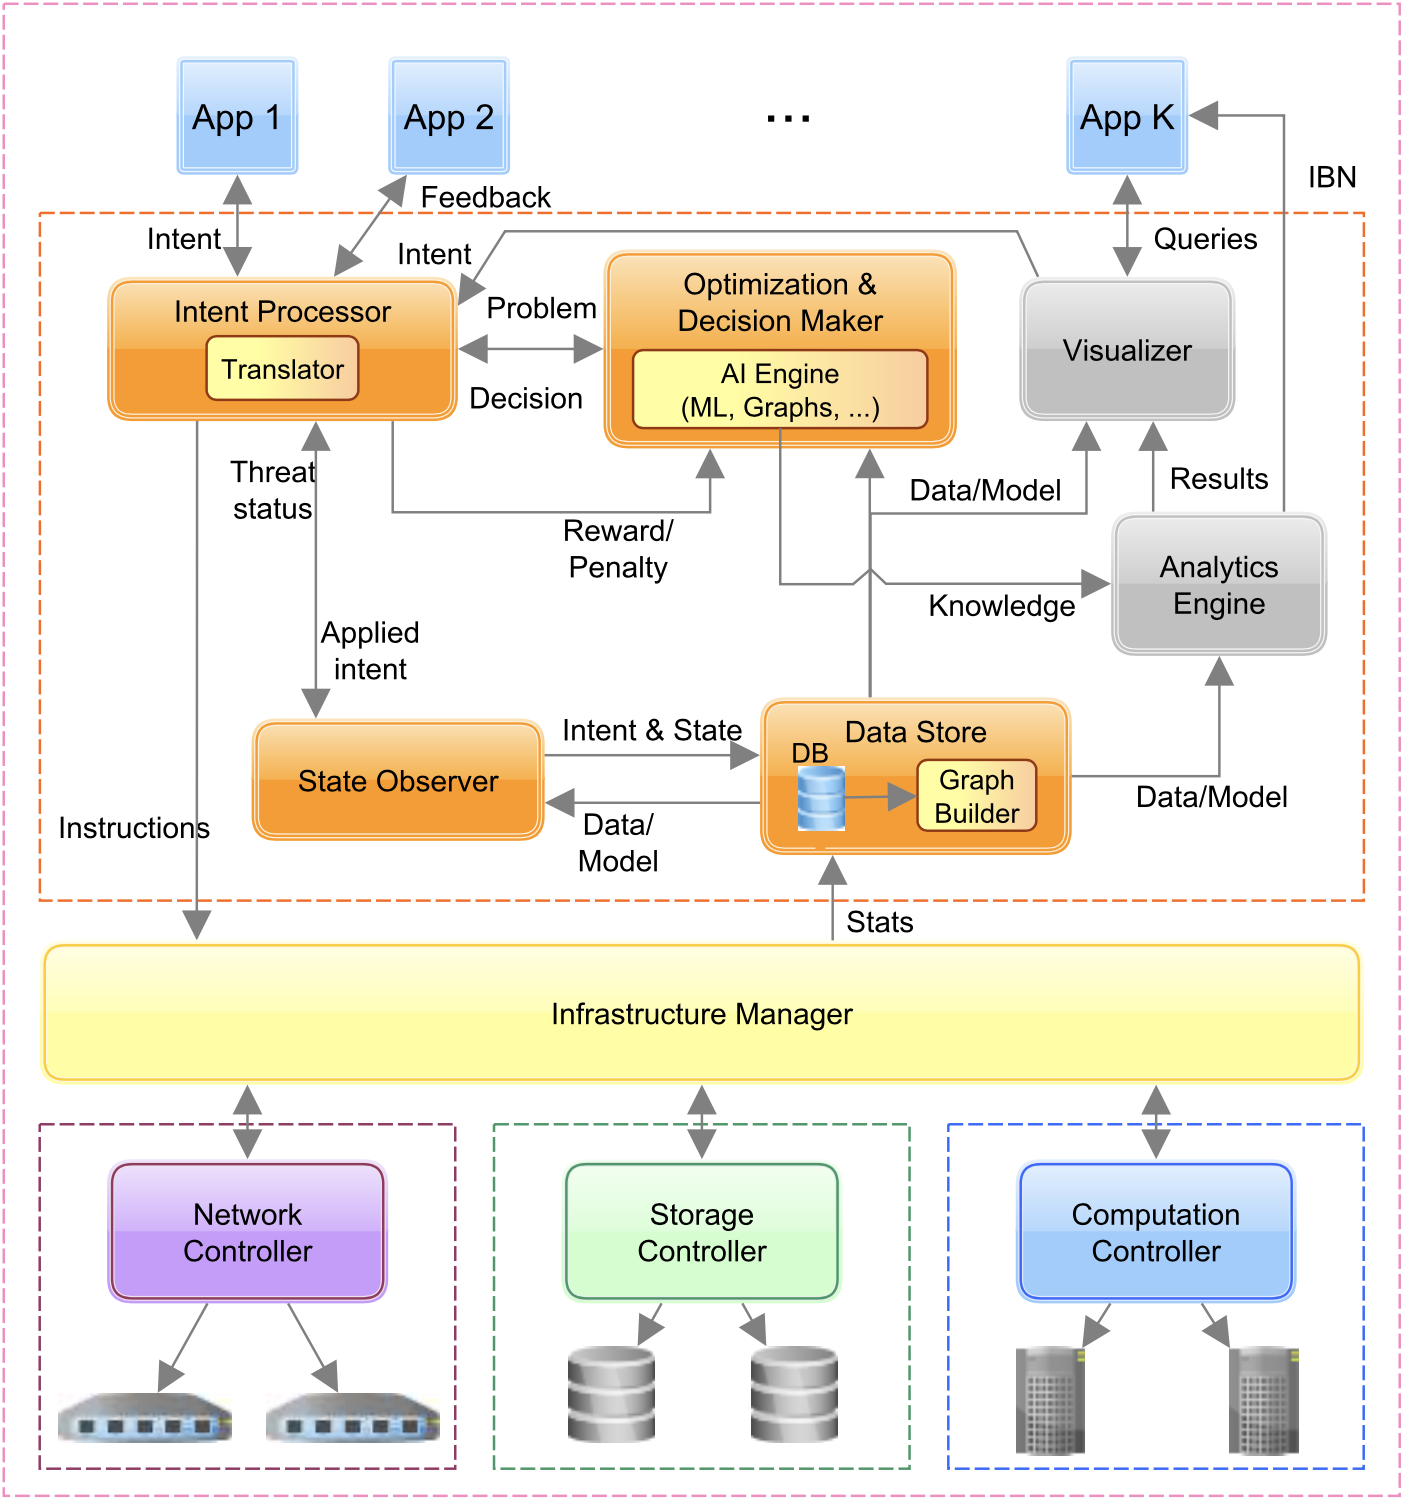
\includegraphics[width=0.7\textwidth]{figures/IBN_Architecture.png}
  \caption{Basic Architecture of IDN\cite{Saha2018}}
  \label{fig:IDN_Architecture}
\end{figure}

\textbf{Intent Processor (IP)} is the core component of IDN architecture that accepts high-level intent provided by users or various applications through a corresponding interface. Intents can be given in different formats, such as simple text, executable commands via a Command-Line Interface (CLI), interaction with a graphical user interface (GUI), or audio interface as speech. After new intent is provided, the translater module performs mapping into a machine-readable representation for the required modules or services. For instance, IP can translate plain text into some internal representation (e.g. Yet Another Next Generation (YANG) as a possible modeling language) with the help of various Natural Language Processing (NLP) technologies\cite[15]{Mehmood2021}. The IP is also responsible for intent assurance. Based on the information from State Observer, IP takes corrective action and assists in the reconfiguration of the underlying infrastructure to preserve the required intents.

\textbf{Optimization Decision Maker (ODM)} is responsible for intent verification optimization and decision making. After receiving as input a mid-level representation of intent, ODM tries to find a feasible and the most optimal solution that is then returned to IP. Based on AI- and ML techniques, the AI Engine (AIE) of ODM learns from past intents to make better decisions in terms of feasibility and intent installation. In addition, this module may be trained on rewards and penalties provided by IP.

\textbf{Data Store (DS)} may store all relevant data collected from the network in a centralized or distributed manner. It provides an API so that other components can store and retrieve data from the DS. Additionally, DS may have a Graph Builder (GB) module that provides a graph view of the underlying network. The graph model can be utilized for optimization, decision making, generating analytics, and network visualization.

\textbf{State Observer (SO)} is a crucial component for intent assurance because it is responsible for monitoring the network. Based on data retrieved from DS it observes the current state and informs IP if there is any threat or inconsistency against installed intent. For instance, a node can be overloaded with network traffic leading to failure in serving a critical service. In this case, the SO identifies the threat and informs the Intent Processor.

The following modules, such as \textbf{Visualizer} and \textbf{Analytics Engine (AE)} are optional components of IDN but still provide some useful functionality. The Visualizer displays information about the state and performance of the network at a glance using a graphical user interface (GUI). It ensures total visibility of the entire network by providing graphical representations of network devices, network metrics, and data flows. Analytics Engine is used to process queries related to network performance, based on raw monitoring data and graph model. Third-party applications may access AE using its API to perform network monitoring.

In IDN, \textbf{applications} are transparent to the underlying system and only interact via appropriate Application Programming Interfaces (APIs) or so-called Northbound Interface (NBI). These APIs play a crucial role as they hide the underlying system's complexities.

The underlying resource layer provides the physical network infrastructure with various device entities. It contains multiple controllers like \textbf{Network (NC)}, \textbf{Storage (SC)}, and \textbf{Computation Controller (CC)} that configure the network devices, such as routers, switches, disks, and servers, according to a required intent. The NC can be an SDN controller or network management system in a traditional network. The \textbf{Infrastructure Manager (IM)} represents an interface between the IP and the different controllers. IM translates feasible intents into domain-specific instructions and also collects various statistics from the controllers.

In comparison, the authors in \cite[13]{Mehmood2021} present another IDN architecture, which is more detailed and contains four following layers: application, intent, network management and orchestration, and resource layers. This survey gives a comprehensive overview of the functions and features of each layer with its key enabling technologies.


\subsection{Intent Translation}

The paper \cite{Jacobs2018} introduces an intent-refinement process that uses machine learning and feedback from the operator to translate intents into network configurations. The proposed refinement method extracts an intermediate representation of intent from natural language before compiling it into SDN commands.

The intent is collected through a chat interface, and a neural network learning model is used to extract entities from natural language. Examples of such entities are the network endpoints, middleboxes, and temporal configurations for the policy. A previously trained sequence-to-sequence learning model based on a Recurrent Neural Network (RNN) with Long Short-Term Memory is used to translate extracted entities to structured intents written in the Nile language. 

Using the Nile language, the operator can build powerful yet simple intents. For example, an input \textit{"Every day from 09:00 to 18:00, the cell should have a range of 1 km with a data rate of 100 Mbit/s, latency under 10 milliseconds and frequency band 2000 MHz"} can be represented as in \Cref{lst:nile_intent_example}. The extracted Nile intent acts as an abstraction layer for lower-level configuration and policy languages. Authors claim the Nile's grammar is expressive enough to represent most network intents.

\begin{lstlisting}[language=Nile,float=ht,caption={Nile intent example\cite{Jacobs2018}},label=lst:nile_intent_example]
define intent qosIntent:
  from    endpoint("cell")
  with    range("equal", "1000m"),
          throughput("more or equal", "100mbps")
          latency("less", "10ms"),
          frequency("equal", "2000MHz")
  start   hour("09:00")
  end     hour("18:00")
\end{lstlisting}

The structured intent definition generated by the translation model is then presented to the network operator for confirmation. The operator may either confirm the correctness of the intent program or make adjustments if necessary. Based on the user’s response, the translation model is then trained, ensuring that the results improve every time the operator provides new intent.

Finally, having a structured intermediate intent representation verified by the user, the Intent Deployer can compile and deploy it into configuration commands using SONATA-NFV, which is an emulation platform that deploys network functions as Docker containers. Decoupling provided by intermediate intent representation ensures the reusability of the proposed solution by allowing compilation of the intents to other existing network configurations and policy languages, such as Janus, PGA, and Kinectic.

However, intent translation is not limited to this implementation. The same paper \cite[20]{Jacobs2018} also briefly covers other existing intent languages, frameworks, and compilers, discussing their goals and shortcomings.
	

\subsection{Industrial Products}

In recent years, the concept of IDN has received great attention from various standardization organizations, open-source communities, and industry. In this section, we present some available IDN solutions.

The European Telecommunications Standards Institute (ETSI) has worked on Experiential Networked Intelligence (ENI) which is a Network Management architecture that uses AI techniques and context-aware policies to address heterogeneous service requirements based on user needs, environmental conditions, and business goals. In terms of open-source solutions, the Open Network Operating System (ONOS) was designed to help network service providers build software-defined networks. ONOS has a component called Intent Framework that allows applications to specify their network control requirements in form of intents. Another open-source project called OpenDayLight also has the Intent Component that enables the controller to manage network services and resources based on generalized and abstracted policy semantics. Also, several industrial companies have developed their IDN products. Cisco has created a digital network architecture (DNA) that is an IDN management platform. Another product Apstra operating system (AOS) is aimed to automate the entire lifecycle of network infrastructure and services. Huawei has announced its IDN solution that will enable SDN-based networks to evolve into IDN-based.\cite{8968429}


\subsection{Advantages of Intent-Driven Networking}

Intent-Driven Networking has clear advantages over regular networking. Most of these advantages lead to significant time savings and improve the agility of the entire system\cite{Kolibri}. The main benefits of IDNs are listed below:\cite[11]{MartinezJulia2022}

\textbf{Simplifies and automates network operations.} IDN reduces the complexity of the management and maintenance of the entire infrastructure. It facilitates work associated with the traditional network configuration and simplifies the deployment of additional network services.

\textbf{Automates troubleshooting and resolution.} Through its closed-loop design, an intent-based network reduces complex troubleshooting scenarios. As assurance processes verify the alignment of network configuration with intent, IDN can recognize potential problems before they occur and immediately perform correcting actions.

\textbf{Enables automatic learning and optimization.} Using machine learning techniques, IDN may predict any violations of the expressed intent before changes will be applied, forecast trends, identify anomalies, predict and validate system-level performance. In addition, IDN may learn from past decisions to determine the most optimal solution.

\textbf{Improves network security capabilities.} Part of the monitoring is that IDN is always looking for threats in the network data. Security violations are immediately identified and prevented.

\textbf{Continuous alignment of the network with the business objectives.} IDN ensures that the network always stays in compliance with the business goals by constantly performing intent assurance and implementation.

\textbf{Fast implementation of business goals into network configurations.} Users can quickly provide high-level business intents, which are then translated into optimal network policies. The configuration of the network components is fully automated.



\section{Challenges of Intent-Driven Networking}

IDN improves the automation of networks and abstracts complex problems, but it also faces some challenges. This section covers several issues that require further research.

\subsection{Lack of standardization}
Different research groups, open-source communities, and industrial companies independently explore and develop IDN solutions. Existing IDN frameworks are based on heterogeneous architectures and underlying techniques that present different functional characteristics. Each component and architectural layer heavily relies on API, and the current unified standard has not been formed. Thus, the absence of a standardized format for specifying intents and common architecture is one of the main challenges of IDN.\cite{8968429}

\subsection{Application of Artificial Intelligence}
The increasing complexity of the mobile networks requires IDNs to be able to translate users' business intents and other requirements into the network configuration, operation, and maintenance policies, and perform the self-configuration, self-optimization, and self-healing of the network. These tasks can be accomplished by AI technologies to ensure network performance while reducing operational costs and improving network robustness. Thus, mobile networks would greatly benefit from advances in the domains of Artificial Intelligence and Machine Learning.\cite{Wei2020}

They are some potential areas that require the integration of AI in the IDN framework:
\begin{itemize}
\item[--] Intent translation.
\item[--] Intent and service assurance with proactive monitoring of resources and network environment.
\item[--] Network planning and configuration.
\item[--] Optimization of the network and service orchestration.
\item[--] Troubleshooting and resolution.
\item[--] Security assurance.
\end{itemize}

Cellular network planning is a challenging process that involves resolving a high number of complex issues, such as uncertainty of input parameters, lack of accurate network details, and complexity of the network. Standard network planning is an iterative process based on approximation techniques with fixed pre-defined inputs. AI techniques like Simulated Annealing, Tabu Search, and Genetic Algorithms can be used to solve complex network design problems, by making more accurate predictions.\cite{anuradha2017empowering}

The self-organizing features including self-configuration, self-optimization, and self-healing play a critical role in the automation of complex networks. For example, a typical 5G node could have thousands of configuration parameters. AI techniques like Transfer Learning, Reinforcement Learning, and Dynamic Programming may be utilized to address configuration management with a highly automated approach.\cite{anuradha2017empowering}

Network monitoring could be challenging in new generation mobile networks due to the dynamic and heterogeneous nature of the cellular environment. With AI-powered diagnostic analytics, the network can quickly and accurately detect problems and resolve them, even before they occur. Based on data from various sources, algorithms like Logistic Regression (LR), Support Vector Machine (SVM), and Hidden Markov Model (HMM) could be utilized for network anomaly detection.\cite{anuradha2017empowering}

The research on the integration of IDNs and AI approaches into mobile networks has just started in recent years. The current studies focus mostly on the core networks, and Intent-Driven mobile networks need further exploration before IDN makes a breakthrough in wireless communication technology, achieving a novel standard in mobile networks.


\subsection{Intent description and translation}
In IDNs, it is expected for the intents to be human-readable at the application level and more machine understandable as the intent flows through the whole system towards the resource layer. The machine-readable format as a mid-level representation is required for efficient intent processing and implementation. However, a human-readable format is preferable for users since arbitrary complex goals can be expressed in a high-level and flexible way. The translation of abstract intents into concrete network configurations is one of the biggest challenge and design goals in IDN systems.

Several different approaches have been proposed for intent representation, such as ontology-based, unrestricted language, vocabulary-restricted, and other hybrid methods. The intent translation is aided by various Natural Language Processing (NLP) technologies. For instance, NLP  can be used for understanding the intent structure and its translation through Sequence-to-Sequence (seq2seq) learning models such as recurrent neural networks (RNN, Long-Short-Term Memory (LSTM), Gated Recurrent Unit (GRU)) and advanced models including attention, Bidirectional Encoder Representations from Transformers (BERT). The context and declarative parameter retrieval leading to the appropriate network configuration can be achieved through a Convolutional Neural Network (CNN). However, the capabilities of these approaches are still limited compared to naturally spoken language. The intent representation and translation problems still have to be explored to provide scalable solutions for human-readable intent description models.\cite[18]{Mehmood2021} 


\subsection{Intent fulfillment and conflict resolution}

From the operator’s perspective, there can be a huge variety of intents. For instance, simple intents that can be fulfilled with a single command on a specific network object or very complex intents that include several commands on multiple network nodes.

The survey \cite{Mwanje2021} presents two methods for fulfilling user-specified intents. The first approach is based on Intent Logic Units (ILU), which may be considered as a wrapper around command sequences or logic that need to be executed to achieve a specific goal. ILUs are stored in an Intent Logic Library (ILL). Intent-Logic Execution Platform (ILEP) retrieves appropriate ILU from the ILL library and schedules its execution. The second method uses Intent-Driven Network Automation Function Orchestrator, which identifies if the intent is valid and executable by Cognitive Automation Network (CAN). Both methods allow the fulfillment of intents but need to be extended in the future to support more features.

To ensure the correct fulfillment of provided intent, IDN should perform its syntactical and semantical validation. Valid intents should still be checked for technical feasibility, in order to avoid conflicts that might occur due to inconsistency, missing network functionalities, or conflicts with existing intents. Infeasible intents should be rejected and the system has to provide an operator with appropriate feedback. Thus, it is necessary to monitor, collect and store network state data and capabilities to perform feasibility checking.

IDN is expected to be provided multiple active intents that should be handled at the same time in an efficient way, leading to various control actions utilizing a shared set of resources. The possibility of conflicts among active intents is unavoidable and requires intent coordination and conflict determination, prevention, and resolution. In order to solve conflicts in network control and management, simple forms of coordination, such as prioritization, partial fulfillment, or queuing were proposed. There are also abstract approaches that use the tools of formal languages and first-order logic to handle conflicts. In addition, the dynamic environment of mobile networks, like the changing number of users and traffic demand, makes this task even more complicated.\cite{Mwanje2021}

Therefore, the detection and resolution of intent conflicts is a major challenge in IDN and needs further research.


\subsection{Legacy networks}
Industries and enterprises tend to move away from legacy network technologies as more efficient solutions become available and the nature of consumer demand changes. However, the legacy network equipment and systems are still often in use. The aspect of migrating them to IDN architecture has to be considered.\cite{Saha2018}


\section{Conclusion}
\label{sec:Conclusion}

In this paper, we discussed Intent-Driven Networking which is the next step toward an autonomous network management system. It gets vast attention from open source communities and industry in recent years. The use of high-level intents simplifies complex network management by offering an efficient and powerful way to manage network infrastructure, resources, and services.

Firstly, we clarified a definition of IDN and presented the corresponding general architecture with its main enabling components. We also covered an intent-refinement process that uses machine learning techniques to translate intents into network configurations. Then we presented available industrial products based on the IDN concept and identified its advantages over regular networking. In addition to the lack of a standardized format for specifying intents and common architecture, IDN faces some challenges in intent translation, fulfillment, and conflict resolution processes. Integration of AI approaches is also a major issue that would enable mobile networks to perform the self-configuration, self-optimization, and self-healing. AI offers powerful algorithms which can be leveraged to manage these challenges. However, more research on AI-enabled IDN needs to be done to improve intelligence in autonomous network operations.

% Literaturverzeichnis
\printbibliography[heading=bibintoc]

% Anhang
\include{appendix}

% Eidesstattliche Erklärung
\clearpage
\section*{\GetTranslation{honesty@title}}
\GetTranslation{honesty@body}

\vspace{2em}
\makeatletter
Augsburg, \@date
\par\vspace{1.5cm}
(\@author)
\makeatother

%%% Local Variables:
%%% mode: latex
%%% TeX-master: "Seminararbeit"
%%% End:


\end{document}